
\label{subsec:ANN:perceptron}

Perceptrons are the simplest topology we can build with artificial neurons. 
Nevertheless, it is the first neural architecture provided with a learning rule,
so the knowledge of the operations behind perceptrons provides a good
basis for understanding more complex networks.

A perceptron neuron uses the hard-limit activation function, which produces a 1 if the net input is equal to or greater than 0; otherwise it produces a 0. 
This function gives a perceptron the ability to classify input vectors by dividing the input space into two regions, which are formed by the decision boundary line at $\mathbf{Wp} + b = 0$ \cite{demuth2008neural}. 
This line is perpendicular to the weight matrix W and shifted according to the bias b 
(notice that hard-limit neurons without a bias will always have a classification line going through the origin).

As shown in \figref{perceptron}, the perceptron network consists of a single layer of 
$S$ perceptron neurons connected to $R$ inputs through a set of weights $\mathbf{W}$. 

\begin{figure}[!ht]
\centering
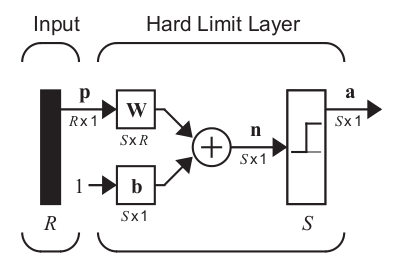
\includegraphics[width=0.6\textwidth]{images/perceptron.png}
\caption{Perceptron network}
\label{fig:perceptron}
\end{figure}

When more than one multiple-perceptron neurons layers are connected, a static feedforward network as the one shown in \figref{neuralnetworkmodelVectorial} is built. 
This topology is called multi-layer perceptron (MLP) and can be trained with the backpropagation algorithm described in \subsecref{staticbackprop}. 
It is known to be a powerful function approximator for prediction and classification problems and it is one of the most commonly used and well-studied ANN architecture.


\subsubsection{Perceptron learning rule}
\label{subsubsec:percpetrontraining}

Its training algorithm belongs to the supervised learning rules group, 
so it makes use of a set of well-known training set $\{\mathbf{p}_1,\mathbf{t}_1\}, ... , \{\mathbf{p}_Q,\mathbf{t}_Q\}$, where $\mathbf{p}_q$ is an input vector of the network and $\mathbf{t}_q$ is the corresponding target output vector. 

For a better understanding of the perceptron learning rule, 
we begin the explanation with a one-neuron network. 
Denoting $e$ as the perceptron error expressed as
\begin{equation}
e=t-a
\end{equation}
where $t$ is the target output and $a$ is the real output of the neuron, the rules that controls the modification of its parameters can be summarised as \cite{Demuth:2014:NND:2721661}
\begin{equation}
\begin{align*}
\text{if } e=1,
\text{then } \mathbf{w}^{\text{new}} = \mathbf{w}^{\text{old}}+\mathbf{p}\\
\text{if } e=-1,
\text{then } \mathbf{w}^{\text{new}} = \mathbf{w}^{\text{old}}-\mathbf{p}\\
\text{if } e=0,
\text{then } \mathbf{w}^{\text{new}} = \mathbf{w}^{\text{old}}
\end{align*}
\label{eq:perceptron3rules}
\end{equation}

Notice that, because we are in the case of a unique neuron, the term of weights $\mathbf{w}$ is a vector and not a matrix. 

Since the sign of $\mathbf{p}$ is the same as the sign on the error $e$ in \eref{perceptron3rules}, its three rules can be unified in a single expression:

\begin{equation}
\mathbf{w}^{\text{new}} = \mathbf{w}^{\text{old}}+e\mathbf{p} = \mathbf{w}^{\text{old}}+(t-a)\mathbf{p}
\label{eq:perceptron1rule}
\end{equation}

This rule can be extended to train the bias by noting that a bias is simply a weight whose input is always 1.
Then, the perceptron rule for the bias is 
$b^{\text{new}}=b^{\text{old}}+e$.

Consequently, for training multiple-neuron perceptrons, the learning rule exposed in \eref{perceptron1rule} can be updated as follows:
\begin{equation}
\mathbf{W}^{\text{new}} = \mathbf{W}^{\text{old}}+\mathbf{e}\mathbf{p}^{T} = \mathbf{W}^{\text{old}}+(\mathbf{t}-\mathbf{a})\mathbf{p}^{T}
\label{eq:perceptron1rule}
\end{equation}
where the superscript $T$ referes to the operation of taking the transpose. Notice that the term of weights $\mathbf{W}$ is now a matrix. The same way, the rule for the bias will be $\mathbf{b}^{\text{new}}=\mathbf{b}^{\text{old}}+\mathbf{e}$.

The aforementioned equations must be applied iteratively until, ideally, the perceptron error becomes zero. In practice, this goal is often impossible, so the algorithm is stopped when the value of the error term $e$ is minumum.



